\DiaryEntry{Depth-First Search}{2020-02-27}{Algorithms}

The depth-first search algorithm searches ``deeper'' into the graph whenever possible. The search explores edges out of the most recently discovered vertex $v$ that still has unexplored edges leaving it. Once all of $v$'s edges have been explored, the search backtracks to explore edges leaving the vertex from which $v$ was discovered. This process continues until all vertices reachable from the source vertex have been discovered.

Slightly different than BFS, the DFS algorithm proceeds if there are still unexplored vertices left: It takes a new source vertex and starts a depth-first search from there. This procedure repeats until all vertices have been visited. Each instance of the DFS algorithm produces a depth-first predecessor tree; in total a forest of predecessor tress is created.

\subsection{Algorithm}

The algorithm colors vertices like the BFS algorithm. It contains of two procedures: The first one (shown below) initialises the data structures (lines 2-4) and then runs over allvertices. If a vertex is white (un-visited) it starts the actual DFS algorithm(lines 6 - 8). It repeats unti all vertices have been explored.

\begin{Verbatim}[numbers=left, xleftmargin=5mm]
DFS(G)
for each vertex u of G
    u.color = WHITE
    u.parent = NULL
time = 0
for each vertex u of G
    if u.color == WHITE
        DFS-Visit(G, u)
\end{Verbatim}

The actual DFS algorithm is shown below. Note that the algorithm assigns two different ``times'' to each vertex: u.d is the time when the node color changed from white to grey (line 3), called \emph{discovery time}; u.f is the time when the node color changed to black (line 9), called \emph{finishing time}. First the node is set to grey (line 4), then it goes over all white adjacent white vertices (lines 5 - 6), sets the parent, and iteratviely calls DFS again (line 8).

\begin{Verbatim}[numbers=left, xleftmargin=5mm]
DFS-Visit(G, u)
time = time + 1
u.d = time
u.color = GREY
for each v in adjacent(G,u)
    if v.color == WHITE
        v.parent = u
        DFS-Visit(G, v)
u.color = BLACK
time = time + 1
u.f = time
\end{Verbatim}

Note that the iteration order of vertices in both procedure DFS and DFS-Visit is not defined and results may depend on the order vertices are visited.

\paragraph{Example.} We consider the following graph as an example.

\begin{figure}[H]
\centering
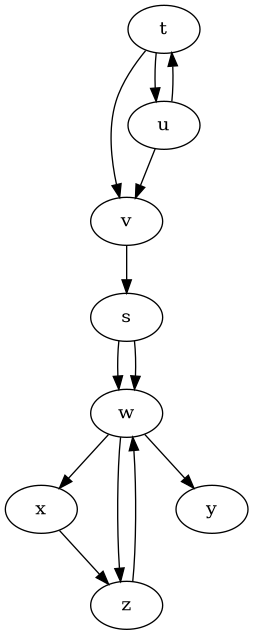
\includegraphics[scale=0.4]{images/dfs_01.png}
\end{figure}

The results of running DFS is shown below. In the implementation of this example, I forced the DFS to start with node $s$ and then $t$. The procedure DFS-visit with root $s$ cannot visit the whole graph as there is no path from $s$ to the ``upper'' part of the graph (vertices $t$, $u$, $v$). So when the DFS-Visit procedure is finished, there are unvisited (white) vertices left. DFS then starts another DFS-visit with $t$ as root and the remaining vertices are visited. In total, two trees are created.

\begin{figure}[H]
\centering
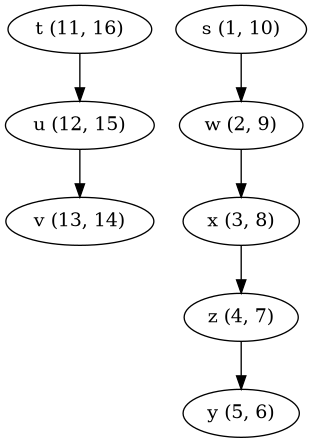
\includegraphics[scale=0.4]{images/dfs_02.png}
\end{figure}

Looking at the intervals created by vertex.d and vertex.f we observe the \emph{parenthesis theorem}: For any two graph vertices $u$ and $v$, exactely one of the following three conditions hold

\begin{itemize}
\item The intervals $[u.d\; u.f]$ and $[v.d\; v.f]$ are entirely disjoint: Then neither $u$ nor $v$ is a descendant of the other in the DFS.
\item The interval $[u.d\; u.f]$ is contained entirely in the interval $[v.d\; v.f]$: Then $u$ is a descendant of $v$ in the DFS.
\item The interval $[v.d\; v.f]$ is contained entirely in the interval $[u.d\; u.f]$: Then $v$ is a descendant of $u$ in the DFS.
\end{itemize}

Looking at our example, we see that e.g. $[u.d\;u.f] = [12\, 15]$ is contained in $[t.d t.f] = [11\; 16]$, therefore $u$ is a descendant of $t$. The intervals $[t.d\; t.f] = [11\; 16]$ and $[s.d\; s.f] = [1\; 10]$ are disjoint; vertices $s, t$ are not descendants of each other.


Let's now modify DFS that it starts with vertex $t$. We achieve the following results shown below. In this case, all vertices are reachable from root $t$, therefore the DFS produces one big tree encompassing all vertices. Note that after the algorithm has discovered vertex $v$, it could have chosen to continue with vertex $w$ instead of $s$. The resulting tree would lookdifferent, but it would stillbe a vlid tree.

\begin{figure}[H]
\centering
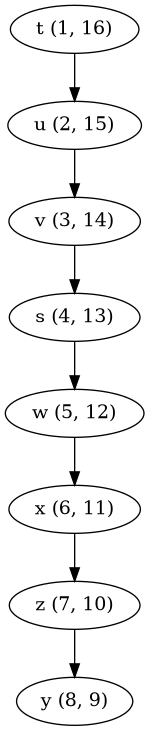
\includegraphics[scale=0.4]{images/dfs_03.png}
\end{figure}

Finally, we consider a slightly different graph as shown below.

\begin{figure}[H]
\centering
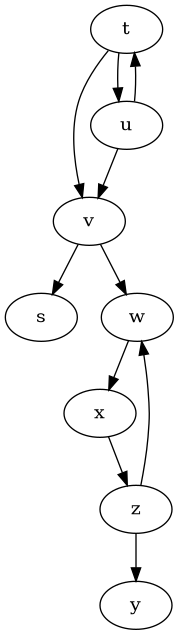
\includegraphics[scale=0.4]{images/dfs_04.png}
\end{figure}

Starting at root $t$, the DFS yields the following tree. The branch at vertex $v$ is interesting: The intervals of $[w.d \; w.f]$ and $[s.d \; s.f]$ are disjoint; they are not ancestors of each other. However, the interal $[w.d \; w.f]$ is contained in $[v.d \; v.f]$ and the interval $[s.d \; s.f]$ is also contained in $[v.d \; v.f]$. So both nodes share vertex $v$ as ancestor.

\begin{figure}[H]
\centering
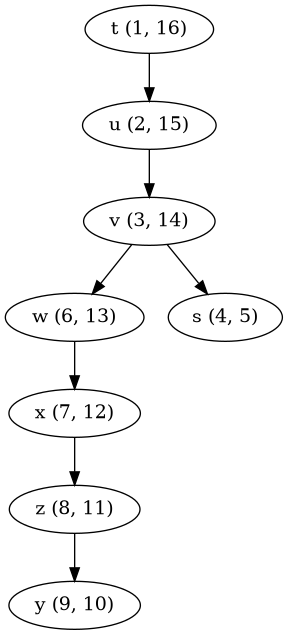
\includegraphics[scale=0.4]{images/dfs_05.png}
\end{figure}


\subsection{Topological Sort}

TBD

\subsection{Strongly Connected Components}

TBD


%%% Local Variables:
%%% mode: latex
%%% TeX-master: "journal"
%%% End:
